
\chapter{Immersion grating process and production}

\section{Heritage}

%\citep{2007ApOpt..46.3400M}
The work I have done on gratings during my 5 year career in the Si diffractive optics group has built upon the decades long effort of the previous generation of researchers.  In this section I briefly summarize the heritage upon which this dissertation has grown.  The most recent refereed publication on the production of our gratings is Marsh, Mar, and Jaffe's 2007 Applied Optics paper titled ``Production and evaluation of silicon immersion gratings for astronomy'' .  The Applied Optics paper came out of Jasmina Marsh's Ph.D. dissertation work, which was almost exclusively on the topic of gratings and grisms.  Jasmina contributed immensely to the current state of production and metrology of gratings.  Katelyn Allers worked simultaneously with Jasmina.  Katelyn's contributions included expanding the grating production to the Pickle Research Campus (PRC) Microelectronics Research Center (most often abbreviated MER, but sometimes also MERC or MRC).  Katelyn characterized the pattern transfer process, specifically in the plasma etch step that we will describe in detail in a later section of this chapter.  Before both Jasmina and Katelyn, Luke Keller was one of the first graduate students who pioneered a lot of the diffraction grating production on wafers.  The institutional memory before Luke has not survived as well.  I overlapped with Jasmina Marsh for about a semester or so.  Casey Deen overlapped with both Jasmina, Katelyn, and me.  Casey was a jack-of-all trades, of sort.  He shepherded the UV exposure system from its old formation to its current form, a metamorphosis described in detail in a later section of this chapter.  Casey also made the initial prototype of our grating efficiency tester, the so-called Custom Robotic Order, Wavelength, and Blaze-Angle Recorder (CROWBAR).  Concurrently with Casey and me, Hyeonju Jeong  was a visiting graduate student for over a year.  

\section{Spin coating}
We use Microposit S1800 series positive photoresist from Microchem.  The S1800 series was historically produced by Shipley, a Boston-area based company, which now appears to be out of business.  The S1800 product is still available through Microchem, which is a distributor for Dow Electronic Materials.  The Microchem website is \url{http://microchem.com/}.  There is not much other information available on the web for this series of resists.  The six-page product guide for the S1800 resists available on the Microchem site is reproduced in its entirety in the appendix for convenience.  There are at least five varieties of the S1800 resists all prefixed with S: 1822, 1818, 1813, 1811, 1805 in order from highest to lowest viscosity.  The resists differ primarily in their viscosity, and therefore the delivered resist thickness for a given spin speed and spin duration.  We do not dilute our resists.

The large size, asymmetric shape, and large thermal mass of our 30 mm thick Si pucks make spinning and baking a challenge.  The spin speed is typically between $\omega=1800-2200$ RPM for 60-90 seconds.  We arrived at these speeds and times by weighing the safety and performance tradeoffs of high angular speeds.  The safety concerns are based on the understanding that a fast rotating mass contains a considerable amount of kinetic energy, which could conceivably be transferred into translational kinetic energy to act as a dangerous projectile.  Specifically we calculate the approximate energy $E$ of a projectile possessing mass $m=550$ g and angular velocity $\omega=2000$ RPM for a solid cylinder with radius $r=50$ mm and height 30 mm.

\begin{eqnarray}
       E&=&\frac{1}{2}I \omega^2 \nonumber \\
		&\sim&15 \textrm{ Joules} \nonumber
\end{eqnarray}

The total kinetic energy of 15 Joules is comparable to a 30 MPH fastball, which is not too bad, but not pleasant either.  Since the energy goes as the square of the angular velocity, a spin speed of 6000 RPM would be 9 times more energy, or a 90 MPH fastball.  We see no performance limitations spinning at 2000 RPM, although we have not experimented on thick substrates at higher spin rates due to safety considerations.  The spin curve for S1805 is included in the Shipley technical document included in the Appendix Section \ref{sec:A1s1800}.  The spin curve for S1805 in that document's Figure 1 shows a film thickness equal to about 600 nm for 2000 RPM spin speed.  Our direct measurements with ellipsometry and stylus profilometry indicate film thicknesses around 600 nm with a 15\% thickness range.  The observed thickness range is consistent with our range of spin speeds and the plot in the Appendix \ref{sec:A1s1800}.

Surface tension effects cause thick buildup of resist, called the edge bead, at the outer few millimeters of the substrate.  The edge bead prevents close contact between the photoresist film and the chrome mask.  Our strategy for edge bead removal is to drag a miniature acetone soaked swab over the outer 2-3 mm.  We explored the performance impact of edge bead removal by comparing two identically prepared wafers with and without edge bead removal.  The wafer that had undergone edge bead removal was uniform upon visual inspection.  The wafer with no edge bead removal demonstrated broken lines over about one third of the wafer surface.  Tests without edge bead removal have resulted in uniformly developed patterns, so edge bead removal probably offers modest advantages some of the time.  Its effect on thick pieces has not been studied in detail, but anecdotally the best piece ever produced in terms of large scale surface flatness, CA1, had edge bead removal performed before contact lithography.  We have no reason to believe that edge bead removal will affect electron beam lithography.  

Figure \ref{fig:spincurve} shows the angular speed as a function of time during spinning.  The recipe pictured has a peak angular speed of 2100 RPM, resulting in a resist thickness of $802 \pm 6 $ nm.  

\begin{figure}[h!] 
\begin{center}
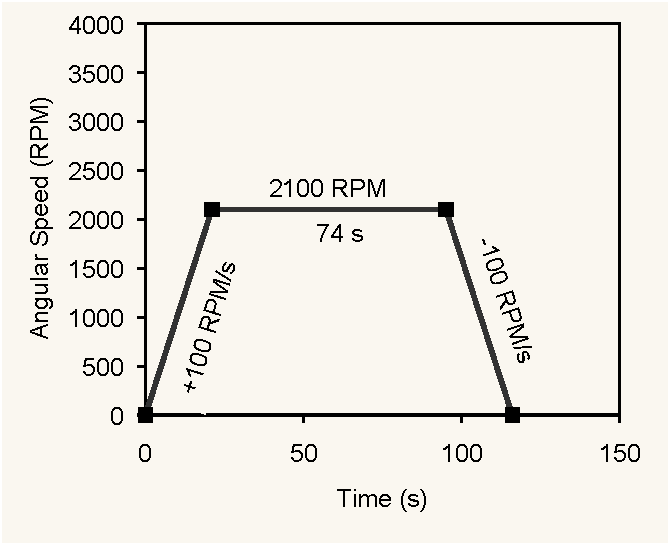
\psfig{file=spincurve,height=2.75in,width=3.25in}
\caption[Photoresist spin curve]{Spin curve for spinning photoresist on massive substrates.  The ramp angular acceleration is 100 RPM/s for 21 seconds, followed by constant angular speed of 2100 RPM for 74 seconds.  The deceleration is 100 RPM/s.}
\label{fig:spincurve}
\end{center}
\end{figure}

\section{Issues related to the photoresist}
Appendix \ref{sec:A1s1800} contains 4 pages from a vendor-provided technical document describing the properties of S1800 series photoresists from Shipley.  Dow chemicals now produces this photoresist under its subsidiary Microchem.  The general behavior of this photoresist should be similar to any positive photoresist, but with slightly different refractive index, resist thickness spin curves, contrast, etc.  In this section we analyze the plots provided in the Shipley technical document to better understand the effect on our UV contact lithography.  The Shipley document largely describes the S1813 photoresist, whereas we use S1805 photoresist.  I am led to believe that these differ only in their dilution, so that they should be identical in all their post-spin bake properties.

\subsection{How to treat ellipsometrically derived thin film thickness}
In this section I rely heavily on measurements of thin film thickness carried out with ellipsometry.  Ellipsometry works by measuring the angular and wavelength dependent elliptical polarization of a small patch (a few mm diameter) of a thin film.  The expected elliptical polarization can be modeled and fitted to the observed data to yield a best fit thickness, or other physical properties that affect the polarization at an interface.  A key aspect of ellipsometry is that you must provide the wavelength-dependent refractive index to accurately fit for the film thickness.  We Cauchy coefficients (XX) provided in Figure 3 of \ref{sec:A1s1800}.  We fit the ellipsometry data in the wavelength range $\lambda = $ 600$-$1000 nm.  We do not fit shortward of 600 nm despite the availability of data to 200 nm.  The reason is that the resist layer is absorptive shortward of 500 nm.  In the range 500 nm to 600 nm, the model fits were poor, suggesting that the refractive index model is especially poor in this wavelength range, which makes sense since the refractive index is a steep function of wavelength in this region.

Our tool is the Woollam M-2000 series ellipsometer.  We have access to two mostly identical versions of this tool, one at the Center for Nano Mechanics (CNM) cleanroom at the UT Austin main campus and another at the Pickle Research Center's Microelectronics Research Center (MRC).  Both tools are in clean environments and function identically.  The CNM tool has a fine adjust translation stage with 2'' range of motion and 0.001'' tick marks on the micrometer scale in both the $x-$ and $y-$ axes.  The MRC tool has no fine adjust translation stage.  We typically sample at intervals of 5\degree angles of incidence in the range 41-76 \degree as measured from the normal to the film surface.

I quantified the impact of changing the refractive index profile to estimate the uncertainties in the film thickness derived with ellipsometry.  Specifically, we computed the thickness derived from the Shipley-provided Cauchy coefficients and the thickness derived from a simultaneous fit to the thickness and refractive index optical constants.  The difference between the two thicknesses derived in this way is typically minuscule (0.3\%), but can be as high as 10\% if the elliptical polarization model fit is poor.  We assigned this uncertainty to the thickness, rather than the much smaller uncertainty reported in the software.  

It is conceivable that there is a systematic error in using ellipsometrically derived film thickness measurements.  We assume that the systematic errors are captured in the uncertainty we assign, and otherwise are negligible.  The biggest concern is the uncertain wavelength-dependent refractive index, which we account for in reporting our uncertainties.  A second less likely problem is that our knowledge of the underlying silicon nitride thickness is uncertain at a 10\% level.  I am led to believe that the thickness of the second layer has negligible impact on the ellipsometric model, and instead it is mostly the interface of the material with the top most thin film that plays a dominant role.  Lastly, we have assumed ideal properties when deriving models of our ellipsometry.  We know that in some cases the resist is non-uniform over the few millimeter beam size, which will smear out polarization signals, but these effects are likely to be miniscule.

\subsection{Do initial variations in the photoresist thickness degrade the grating performance?}
In this subsection I answer the question ``to what extent do initial variations in the photoresist thickness contribute to performance degradation?''.  Anecdotally, the resist coating process must be fairly uniform since spin-coated wafers have the same color photoresist everywhere- if there were dramatic thickness variations we would see different colors, like when there is a comet that messes up the photoresist.  To check our intuition, I directly measured the photoresist thickness in 5 different points on a spin-coated but unexposed wafer.  I measured the resist thickness with the Woollam M-2000 series ellipsometer at CNM.  The wafer was prepared with our usual recipe with the spin curve shown in Figure \ref{fig:spincurve}.  The thickness in the center was 806.9 $\pm$ 2.6 nm, while at a location 2.8'' away the thickness dropped to 799.7 $\pm$ 1.8 nm.  The uncertainties in the difference of resist thickness are much less than the systematic error reported, so the trend and level of the difference is firm.  The peak to valley variation of our 5 data points is 0.9\%.  The resist is remarkably uniform.  Still, the phenomena of interference and high contrast in photoresists means that we have to convert the level of this initial thickness variation into an exposure time difference in order to rule out initial film thickness as a source of performance degradation in immersion gratings.

Figure 4 in \ref{sec:A1s1800} shows a plot of interference curves ($E_0$ vs thickness, where $E_0$ is the critical dose) for our resist in the thickness range 1100-1400 nm.  Our $\sim$800 nm resist thickness is well outside this range.  I performed a by-eye fit to the data including a sine wave with a linear and constant term: $E_0=A\sin(2\pi [t-t_0]/T) + Bt+C$.  I extrapolated this fit past 800 nm.  Figure XX shows the digitized data points from Figure 4 in \ref{sec:A1s1800} in red, my fit to those data points in blue, and the extrapolation in yellow.  This strategy is highly uncertain- I do not even know if my model of a sinusoidal variation is accurate.  With that proviso, the fit looks fairly convincing, and 800 nm is right on the part of the interference curve with the maximum slope.  This means our choice of resist thickness (more specifically, our choice of maximum spin speed), is unfortunate.  The minute variations in initial resist thickness are amplified in the requisite dose to clear.  One glaring problem with my model is the direction of the variation is all wrong- the observed resist is thicker in the middle than the edge, whereas my model predicts that the center should have a lower critical dose and therefore be thinner than the edge.  There are a few places why this model failed.  First, my projection is probably not accurate.  Second, the data is for the case of G-line only UV illumination, whereas the spectrum of our UV lamp (c.f. Figure XX) has a broad spectrum of other bright lines which will wash out the sharp peaks of Figure \ref{fig:S1800interference}.   

\begin{figure}
\begin{center}

\subfloat[Projected photoresist interference curve]{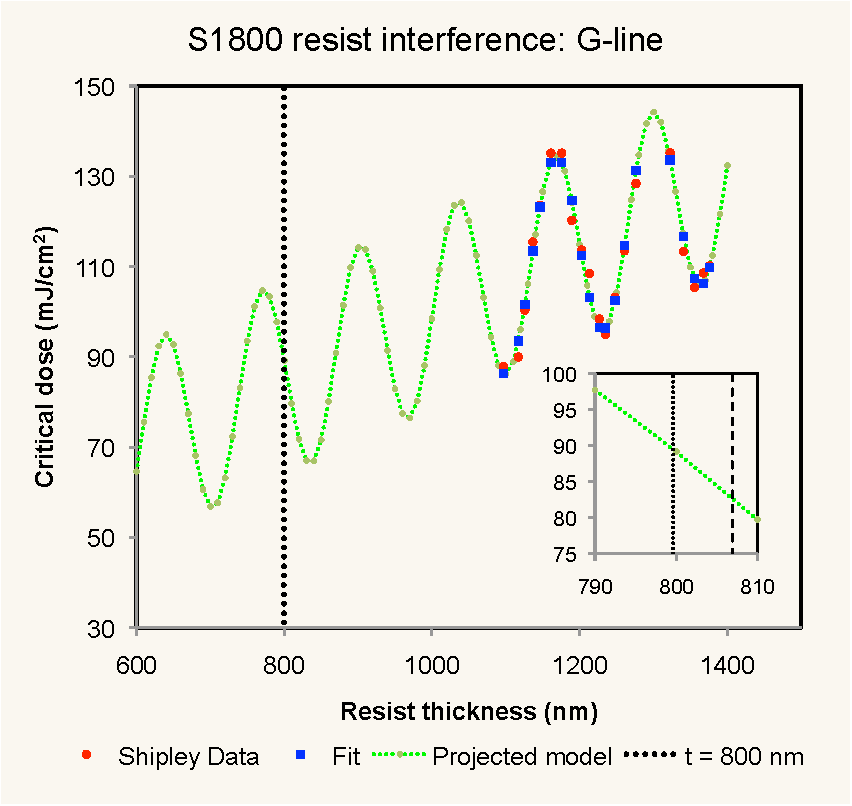
\psfig{file=chGratingProcess/S1800interference.pdf,height=2.75in,width=3.25in}}
\\
\subfloat[Center to edge variation assuming the projected interference]{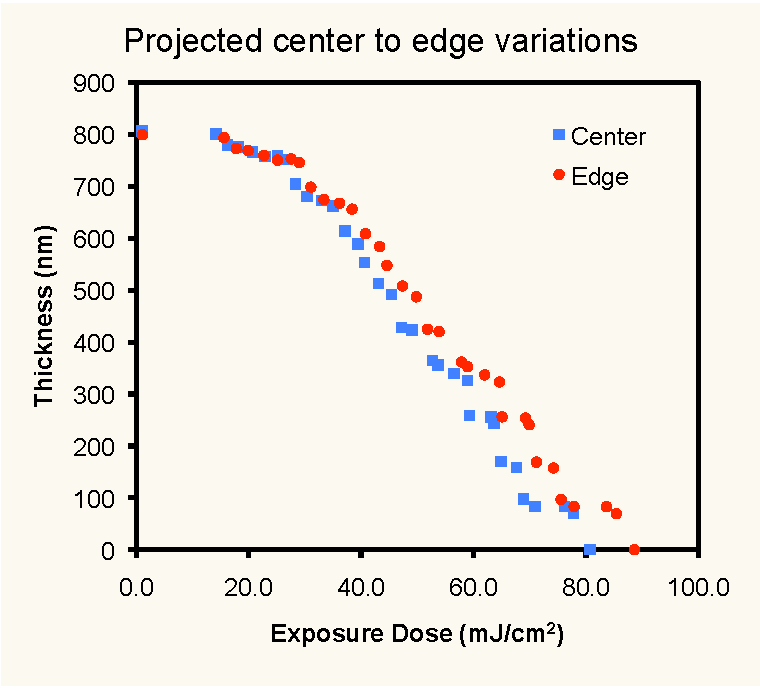
\psfig{file=chGratingProcess/projectedC2Evariation.pdf,height=2.75in,width=3.25in}}
\caption[Projected photoresist interference]{The projected photoresist interference assuming mercury G-line wavelength exposure.  The inset shows a blow-up of the thickness range surrounding the thickness of our photoresist, 800 nm.  The thickness of our resist ranges from 807 nm at center to 800 nm at edge, which corresponds to a projected critical exposure difference of 82 mJ/cm$^2$ to 90 mJ/cm$^2$.}
\label{fig:S1800interference}
\end{center}
\end{figure}

The second panel of Figure \ref{fig:S1800interference} shows the estimated thickness as a function of dose for the case of the center thickness 807 nm and edge thickness 800 nm, with the projected interference from the first panel of the same figure.  The 0.1\% difference in resist thickness can translate into a 60-80 nm difference for otherwise identical exposure time.  With my assumptions of the interference curve, the locations where the resist is initially thinner will actually stay thicker longer, owing to their larger critical dose to clear.  This result is a little bit shocking, but remember this is an upper limit on the effect, assuming maximum slope on the interference curve.  It is worth investigating to what extent our resist is monochromatic or broadband.  In the next section we seek to answer this question.

\section{Which wavelength range is most effective in illuminating the resist?}
The delivered dose depends on the spectral characteristics of the UV light source and the absorption properties of the resist.  I computed the product of these curves to construct the absorbed power as a function of wavelength.  I digitized the S1800 absorption as a function of wavelength curve in Figure 6 of the Shipley technical document in \ref{sec:A1s1800}, only for the unexposed resist curve.  I smoothly extrapolated the absorption past 500 nm, assuming 0.1\%absorption for $\lambda > 535$ nm.  I similarly digitized the vendor-provided UV spectrum of the Omnicure 2000 lamp, which I accessed from the Omnicure website.  I interpolated both curves onto a wavelength scale from 250$-$700 nm at 2.5 nm intervals, then took the product of the curves.  The result is shown in Figure \ref{fig:UVabsSPEC}.  It appears that all three strong UV mercury lines (I-, H-, and G- lines; 365, 405, 436 nm) contribute to the exposure of the resist.  The polychromatic exposure questions the assumption of using the curves provided in the Shipley technical guide, since the guide explains that the illumination source is G-line only.  In our plot, the G-line accounts for a small fraction of the power.  

\begin{figure}[h!] 
\begin{center}
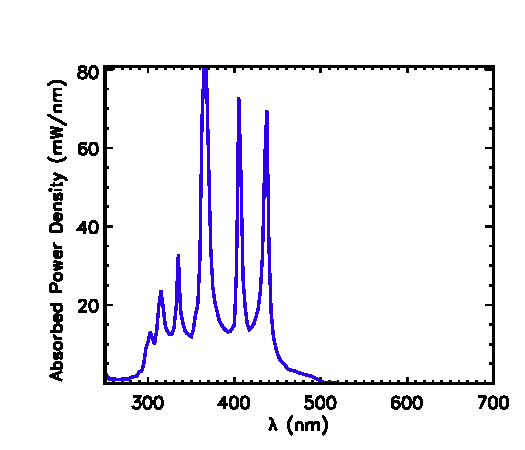
\psfig{file=chGratingProcess/UV_spec_abs.pdf,height=3.0in,width=3.50in}
\caption[UV absorption and lamp spectrum]{The absorbed power density as a function of wavelength.  This curve is the product of the lamp wavelength and the absorption of the S1800 photoresist.  See the text for the assumptions and extrapolations.  The line at 435 nm is the mercury G-line.  It is clear that the other lines contribute strongly to the delivered dose of the S1800 photoresist.  These other peaks should smear out the interference curves shown Figure \ref{fig:S1800interference}.}
\label{fig:UVabsSPEC}
\end{center}
\end{figure}



\section{UV mask contact lithography}
Figure \ref{fig:uvsys} shows a schematic of our UV contact photolithography system.  The UV light source is an Omnicure S2000.  The Omnicure spectral properties have not been independently verified, but are shown in Figure \ref{fig:UVabsSPEC} as the product of the unexposed absorption of the photoresist and the lamp output.  The S1805 photoresist is optimized for mercury G-line (435.8 nm), but it is effective with broadband exposure.  The major property of photoresists is their critical polymerization upon exposure to UV light.  In the positive photoresists like the S1805 we use, the area exposed to UV light is polymerized, and develops away.  The area shadowed by chrome masking remains.  Figure 7 in Appendix \ref{sec:A1s1800} shows how the normalized photoresist thickness remaining depends on the delivered dose.  One major property we care about is the so called ``dose to clear'' or ``critical dose'', denoted as $E_0$ in Figure 7 in Appendix \ref{sec:A1s1800}.  The critical dose is an intensity above which the photoresist is polymerized and below which there is no change in the photoresist properties.  An ideal binary resist will have an infinitely sharp transition- a step function- from cleared to uncleared.  Real-world resists have a finite and gradual transition from uncleared to cleared.  Specifically, the post-development resist thickness will monotonically decrease as a function of exposure until it reaches the critical dose, and then no further reactions will take place.  The chemistry of how this reaction takes place is beyond the scope of this report, and is summarized elsewhere (cite XX).  Suffice it to say, photoresists of all varieties have been created to have a variety of properties.  


\begin{figure}[h!] 
\begin{center}
\ 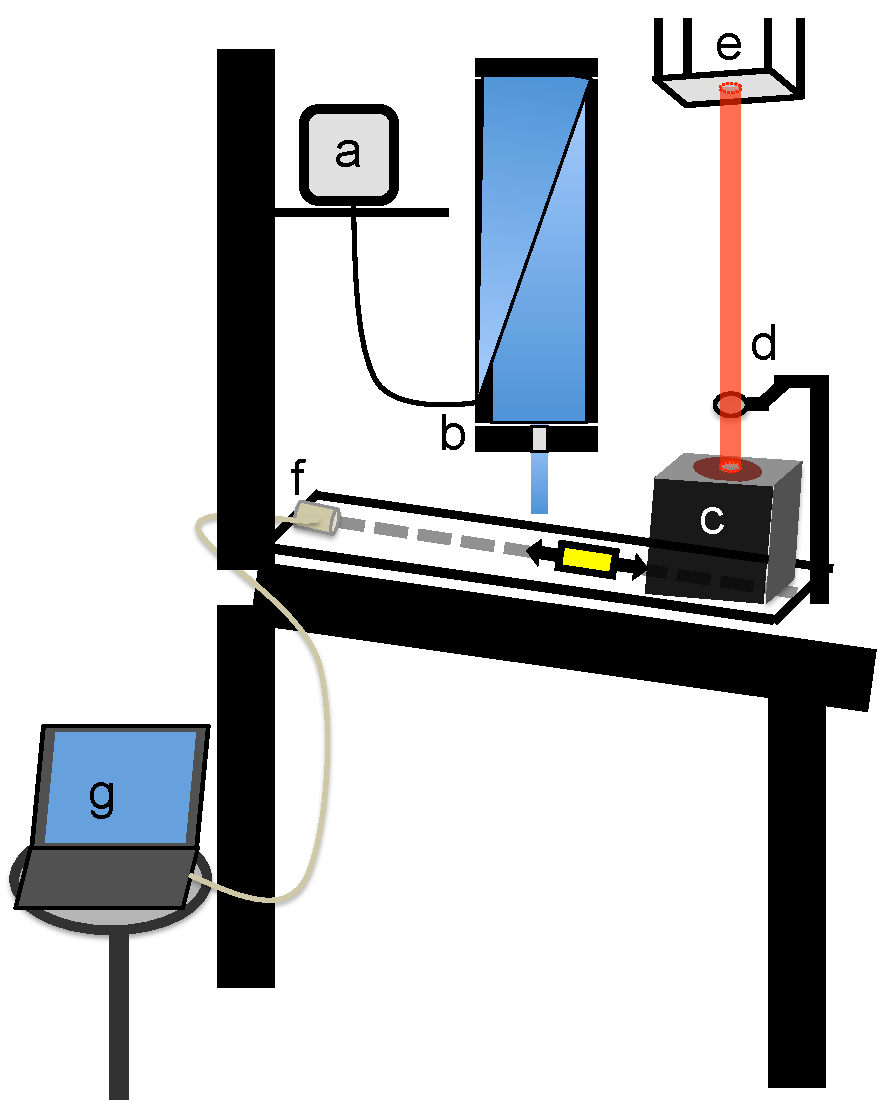
\psfig{file=chGratingProcess/UV_expos_graphic2.pdf,height=4.5in,width=4in}
\caption[Schematic of our UV exposure system]{Schematic of our UV exposure system.  The UV exposure system operates by moving the mask-substrate unit beneath a stationary UV light source.  The key components of the system are labeled.  The ultra stable UV lamp (a) is fiber fed to a collimating mirror, before passing through a 1'' $\times$ 6'' slit (b) with its long axis perpendicular to the direction of motion of the car (c).  A 632 nm laser beam (d) illuminates a 1'' diameter beam on the mask-substrate unit to aid in minimizing Newton's rings fringes from poor contact.  The beam is viewed on a white card (e).  A computer controlled motor (f,g) controls the delivered exposure dose by defining the rate of motion and number of passes for the car.}
\label{fig:uvsys}
\end{center}
\end{figure}

\begin{figure}[h!] 
\begin{center}
\ 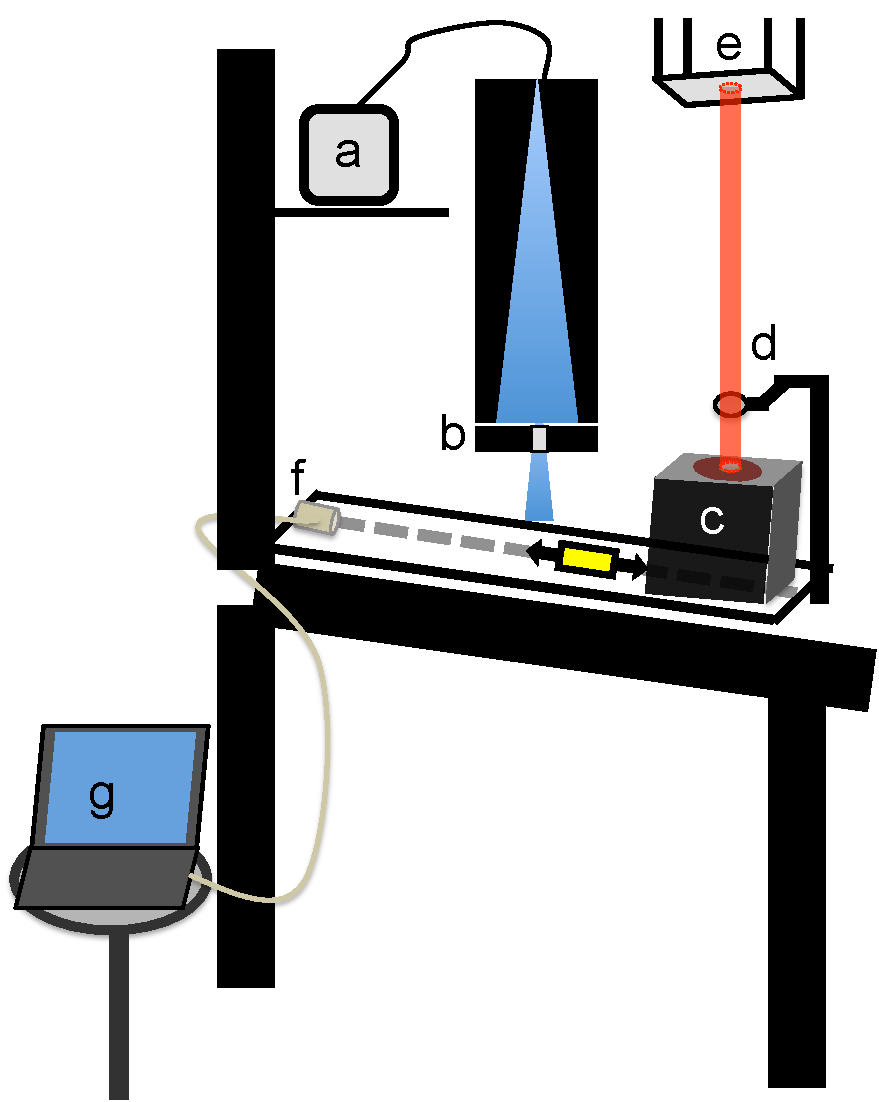
\psfig{file=chGratingProcess/UV_expos_graphic1.pdf,height=4.5in,width=4in}
\caption[Schematic of our former UV exposure system]{Schematic of our setup for the UV exposure system before 2010.  The key difference of the previous exposure system and the current system is the strategy for illumination, specifically collimation.  In the old system we simply had the light guide directed downward from the top of the tower, whereas in the new system we have a mirror at the top of the tower to receive the divergent beam from the light guide and subsequently collimate the beam toward the slit.}
\label{fig:uvsys}
\end{center}
\end{figure}

Our main concern with photoresist has to deal with where exactly the position of the critical dose is met in the vicinity of the chrome line edge position.  There are a variety of factors that contribute to the critical dose position.  Figure \ref{fig:dose2clear} shows the normalized thickness of resist as a function of exposure dose.  We constructed this photoresist contrast curve by exposing a resist coated wafer without a lithographic mask.  We masked 14 subregions of the wafer with a red film, exposures ranging from 36 to 0 passes.  Figure XX shows a photo of the wafer demonstrating the apparent non-uniformities.

\begin{figure}[h!] 
\begin{center}
\ 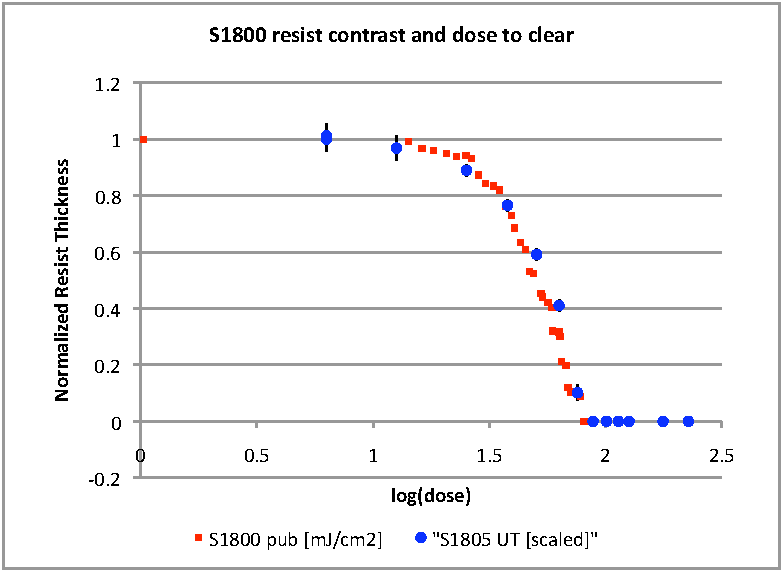
\psfig{file=chGratingProcess/dose2clear.pdf,height=4in,width=5.5in}
\caption[S1800 photoresist contrast curve]{S1800 photoresist contrast curve.  The red points are digitized values from Figure 7 of the Shipley S1800 series photoresist guide.  The $x-$ axis is the log of the exposure dose in mJ/cm$^2$.  The blue points are UT lab-measured values in number of passes plus a constant $x$ offset to match up with the scale on the Shipley measured values.  We know from the Shipley report that their values are for S1813 resist thickness 1230 nm, whereas our S1805 resist thickness is 700 nm, so we do not expect the dose to clear to be equal for these two different cases.  In fact, Figure 4 in the Shipley product guide shows that the dose to clear, $E_0$, can vary by 50\% for an 8\% change in resist thickness.}
\label{fig:dose2clear}
\end{center}
\end{figure}


\begin{figure}[h!] 
\begin{center}
\ 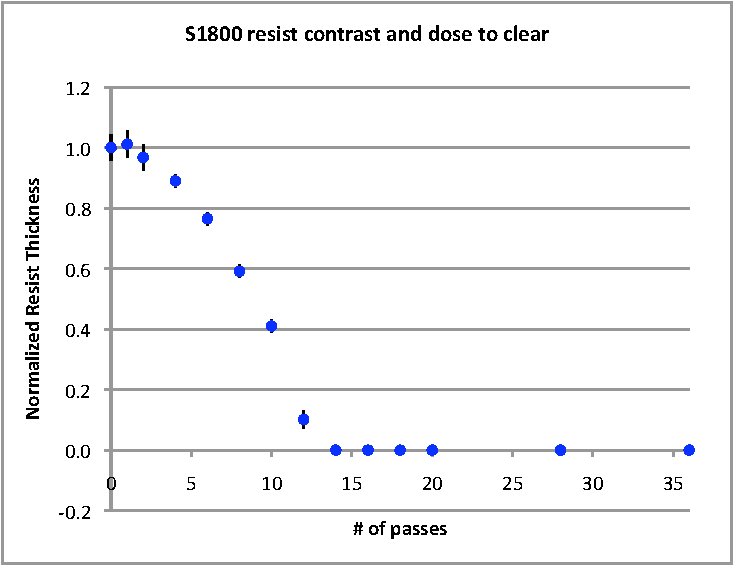
\psfig{file=chGratingProcess/dose2clear2.pdf,height=4in,width=5.5in}
\caption[Experimental photoresist contrast curve]{Photoresist contrast curve in units of number of passes on a linear scale.}
\label{fig:dose2clear2}
\end{center}
\end{figure}


\begin{figure}[h!] 
\begin{center}
\ 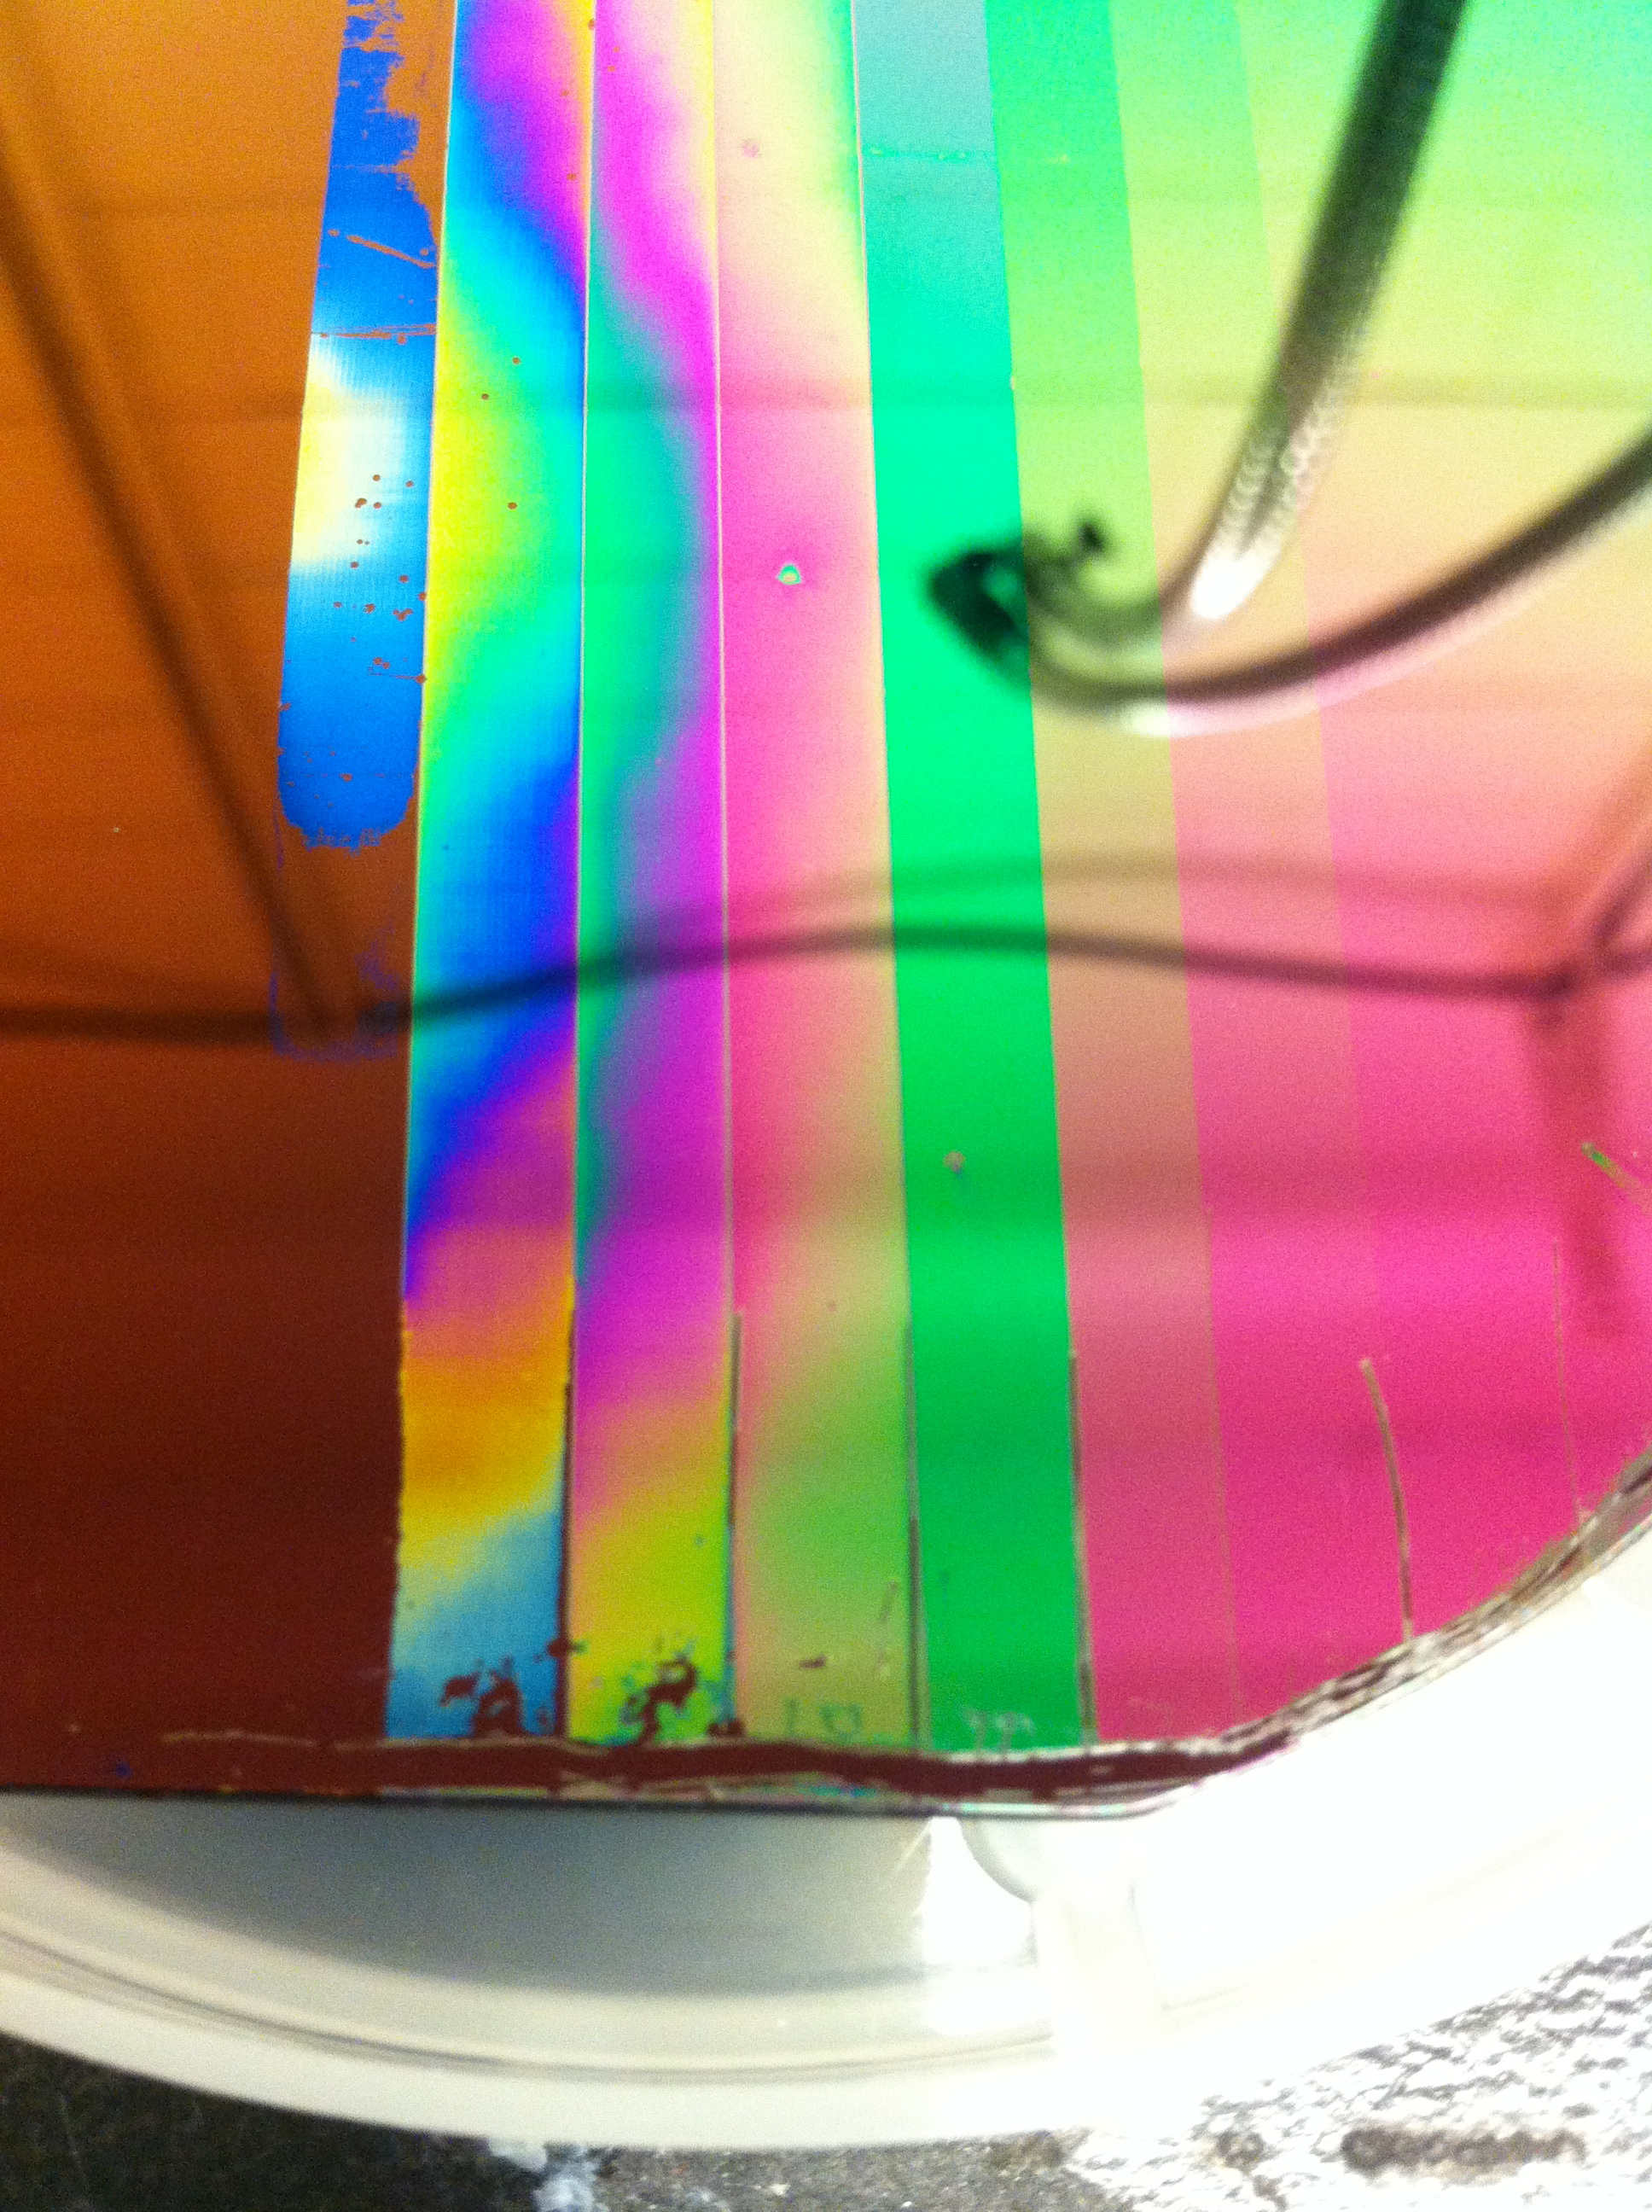
\psfig{file=chGratingProcess/IMG_3285.jpg,height=5in,width=4in}
\caption[Photo of experimental wafer]{Photo of the wafer used to make figures \ref{fig:dose2clear2} and \ref{fig:dose2clear}.  The large scale non-uniformities are apparent at the region near the critical dose.}
\label{fig:dose2clearphoto}
\end{center}
\end{figure}

\begin{figure}[h!] 
\begin{center}
\ 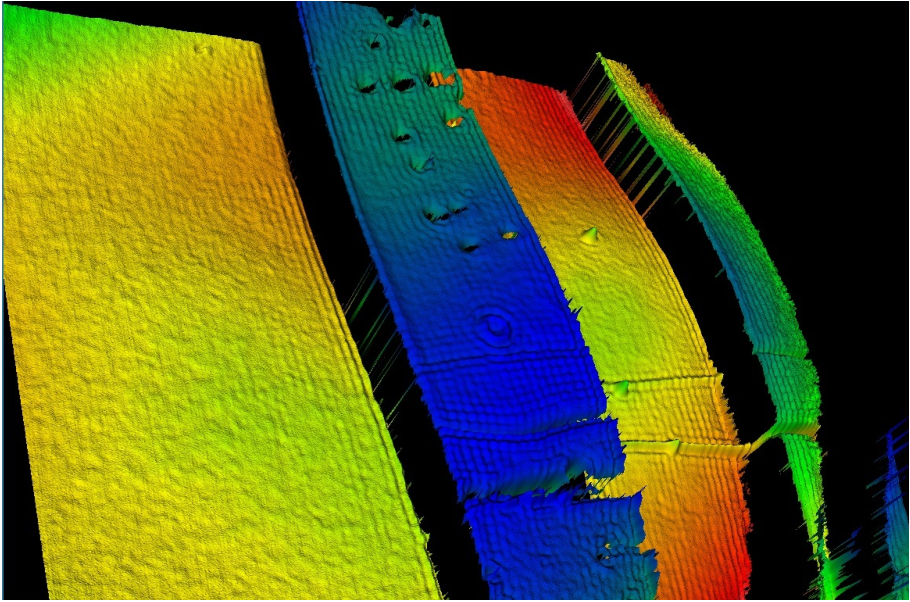
\psfig{file=chGratingProcess/3Dzoomw20120926.pdf,height=5in,width=6.25in}
\caption[Zygo interferometry of experimental wafer]{Zygo interferometry at maximum zoom.  The target is the wafer shown in the photo in Figure \ref{fig:dose2clearphoto}, centered around the region near the critical dose.  The 3D map shows fine spatial structure that is barely perceptible.  The steps are approximately 5 mm wide.  }
\label{fig:3dZYGOresist}
\end{center}
\end{figure}

The UV exposure step is probably the most critical and most mysterious step in our device production process.  In the subsection below I will enumerate some of the dominant unknowns in the UV exposure step.  Part of the reason why there is some mystery in the system is because experiments are costly in hardware and effort.  Consumable and costly thick Si pucks are required to probe the quality of contact, since wafers are too flexible.  Experiments with thick pieces are often inconclusive anyways, given the large amount of uncontrolled variation in other parts of our process and the small number of experiments, owing to the per-part cost.  Consider the following example.  In the summer of 2011 Dr. Weisong Wang and I were seeking to make the iSHELL LM immersion grating on the recently overhauled exposure system.  The overhaul had improved the UV beam collimation but the system suffered an 80\% light loss as a result.  Our first experiment E\#\# (XX)  yielded a peak to valley surface error of about 0.8 waves over a 25 mm beam at R3.  Weisong and I proposed that the exposure dose was insufficient, and we were merely operating in the exposure regime near the critical dose where minute changes in the dose are amplified into large position deviations of line edges.  Our solution was to try exposing another part with a longer exposure time.  So we made part (E\#\# XX), which demonstrated identical performance to the previous (poor) E\#\# (XX).  There was no change in performance.  What did we learn from this series of experiments?  The per-part cost of thick pieces is prohibitive, which we already knew, but appreciated more after a part was spent in vain.  We learned that it is better to design an experiment that will unambiguously answer which effect is dominant among our milliard steps.  For example, we did not necessarily find out that the exposure time was not to blame, given that we simply could have still been near the critical dose regime- that is, maybe we just did not increase our dose enough.  


There are many unknowns in the UV exposure step.  How good is the contact between the photolithographic mask and the Si substrate?  Does the contact change with time and temperature?  Specifically, does the movement of the car jostle the mask and substrate with respect to each other?  What is the degree of collimation of the UV beam?  What is the profile of the beam along the length of the slit, and more generally what is the 2D beam uniformity?  Does the profile of the beam along the length of the slit change in time?  Does the UV lamp intensity change in time?  To what extent is the beam non-uniform; how does the uniformity compare to vendors of mask aligners.  How does dose variation translate to a phase error?  Does the lamp have periodicity on short timescales ($\tau < 10 $ s) that will appear as periodic linewidth variations?  Similarly, does the lamp have long term drift so that the exposure time is lengthening or shortening in time?  Does firm contact between the mask and substrate peel off some of the photoresist, causing point defects?  Does resist from previous contacts stick to the mask and prevent good contact on future trials?  How good is the mask to begin with?  What is the UV sensitivity spectrum for the resist we are using?  What is the delivered intensity of our UV exposure system?  What is the dose?  What is the process latitude for our combination of developer concentration, dose, develop time?  Should we use a post-exposure bake?  Do we see standing waves in the vertical cross sections of our resist features?  Is there anything to gain by changing the spectral properties of the illumination, namely more or less bandwidth, or longer or shorter average wavelength?

\subsection{What is the beam intensity uniformity?}
The beam intensity spatial uniformity is important because the minuscule intensity variations implant phase errors in the resist sidewalls which translate into phase errors in our gratings.  Our dilemma is similar to taking a flat field during astronomical calibrations.  How uniform can a light beam be made?  The industry standard is the mask aligners of Karl Suss and others.  Suss specifies the UV illumination uniformity in their product datasheets available on their website \url{http://www.suss.com/en/products-solutions/products/mask-aligner/ma300-gen2/overview.html}.  For example, the MA300 Gen-2 has an intensity uniformity of 3-5\% depending on the wavelength chosen, but it is important to note that this uniformity is over the 12 inch diameter for their large wafers.  The uniformity over the inner 4 inches must be much better than 3\%, probably 1\% or better.  At the time of writing, our group does not have a good way to directly measure the UV-intensity uniformity.  

We have indirect detection of non-uniformity from the grayscale lithography of un-patterned wafers.  The method is described in detail in other sections in this chapter.  It is not safe to attribute the observed morphology entirely to the beam intensity nonuniformity, since the initial film thickness and the development process are likely to contribute to the non-uniformity as we will show in the next sections.  Still we can estimate the non-uniformity by positing that the lion's share of the morphology seen in grayscale tests is from the exposure process.  With this assumption, the range in resist film thickness is indicative of the range in UV exposure.  Figure 2.6 shows the vendor-provided dose-to-clear curve we have verified with our resist and substrate configurations.  Figure 2.7 shows the same measured curve on a linear scale.  Ellipsometry of grayscale exposed wafers shows that 80\% of the wafer surface has a resist film thickness in the range of 40 to 250 nm.  The initial film thickness is about 700 nm, so the normalized thickness variation is 5$-$35\%.  This magnitude of thickness variation corresponds to 18\% in UV dose non-uniformity.


\subsection{High spatial frequency structures in gratings}
High spatial frequencies in the context of our grating manufacturing are those structures that produce peaks in a monochromatic spectral impurities separated by a few diffraction widths, say $>5$ or so.  For a 25 mm beam, periodic structures with periods of 5 mm or less are considered high frequency.

One source of high frequency structures is the vibration of the turret and the car as the motor drives it forward.  Table xx summarizes the measured properties of the UV exposure system motion.  We measured the high frequency vibrations by resting an accelerometer on the fine adjust translation turret.  The STMicro STM33H 3-axis accelerometer was sensitive to frequencies of 0.1$-$40 Hz, with a target sample rate of 100 Hz, although we typically achieved only 90 Hz.  We sampled 2048 measurements over about 22 seconds.  We measured an RMS acceleration of 0.002 $g$ in the $x-$axis when the motor was at rest.  We tabulated the vibration frequency and amplitude for driving frequencies of 25, 43, 50, 67, and 200 rpm.  Figure XX shows the frequency and amplitude response of the motor for the range of driving frequencies.  

How does the vibration manifest in the exposure?  The linear position of a point on the wafer as a function of time is given by:

\begin{eqnarray}
 x(t)= x_0 + v_0 t + A \sin(2\pi f t - \phi)      \nonumber \\
 0 < x_0 < 100 \text{ mm}
\end{eqnarray}

Where the average speed $v_0$, amplitude $A$, and frequency $f$ comes from Table XX, and $\phi$ is arbitrary.  The UV slit width is 1".  The vibrating wafer slides under the UV slit, imprinting the phase difference of the entrance and egress from the light beam as a tiny exposure time difference that is periodic.  The period is about 210 $\mu$m, with an ans Figure XX shows a schematic of the processes, the position of a point on the wafer as a function of time, and the calculated effect for slit width equal to 25.35 mm.  

\begin{figure}[h!] 
\begin{center}
\subfloat[Schematic of the Wafer and UV slit motion]{\ 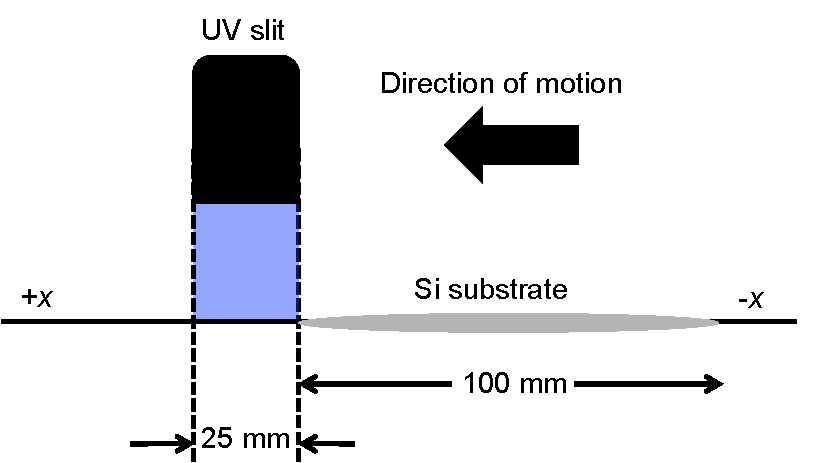
\psfig{file=chGratingProcess/UV_slit.pdf,height=2in,width=3in}}
\\
\subfloat[Vibration effect on position and dwell time]{\ 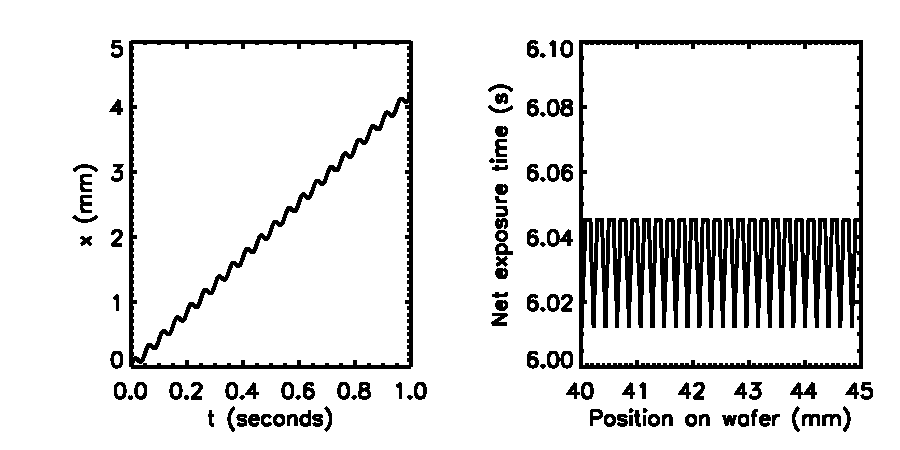
\psfig{file=chGratingProcess/UV_vibrations.pdf,height=3in,width=6in}}
\caption[Motor vibrations schematic]{The effect of vibrations is to produce periodic exposure dose as a function of position.  The period is about 210 $\mu$m, which is equal to the observed frequency.}
\label{fig:uvvibs}
\end{center}
\end{figure}

\begin{figure}[h!] 
\begin{center}
\ 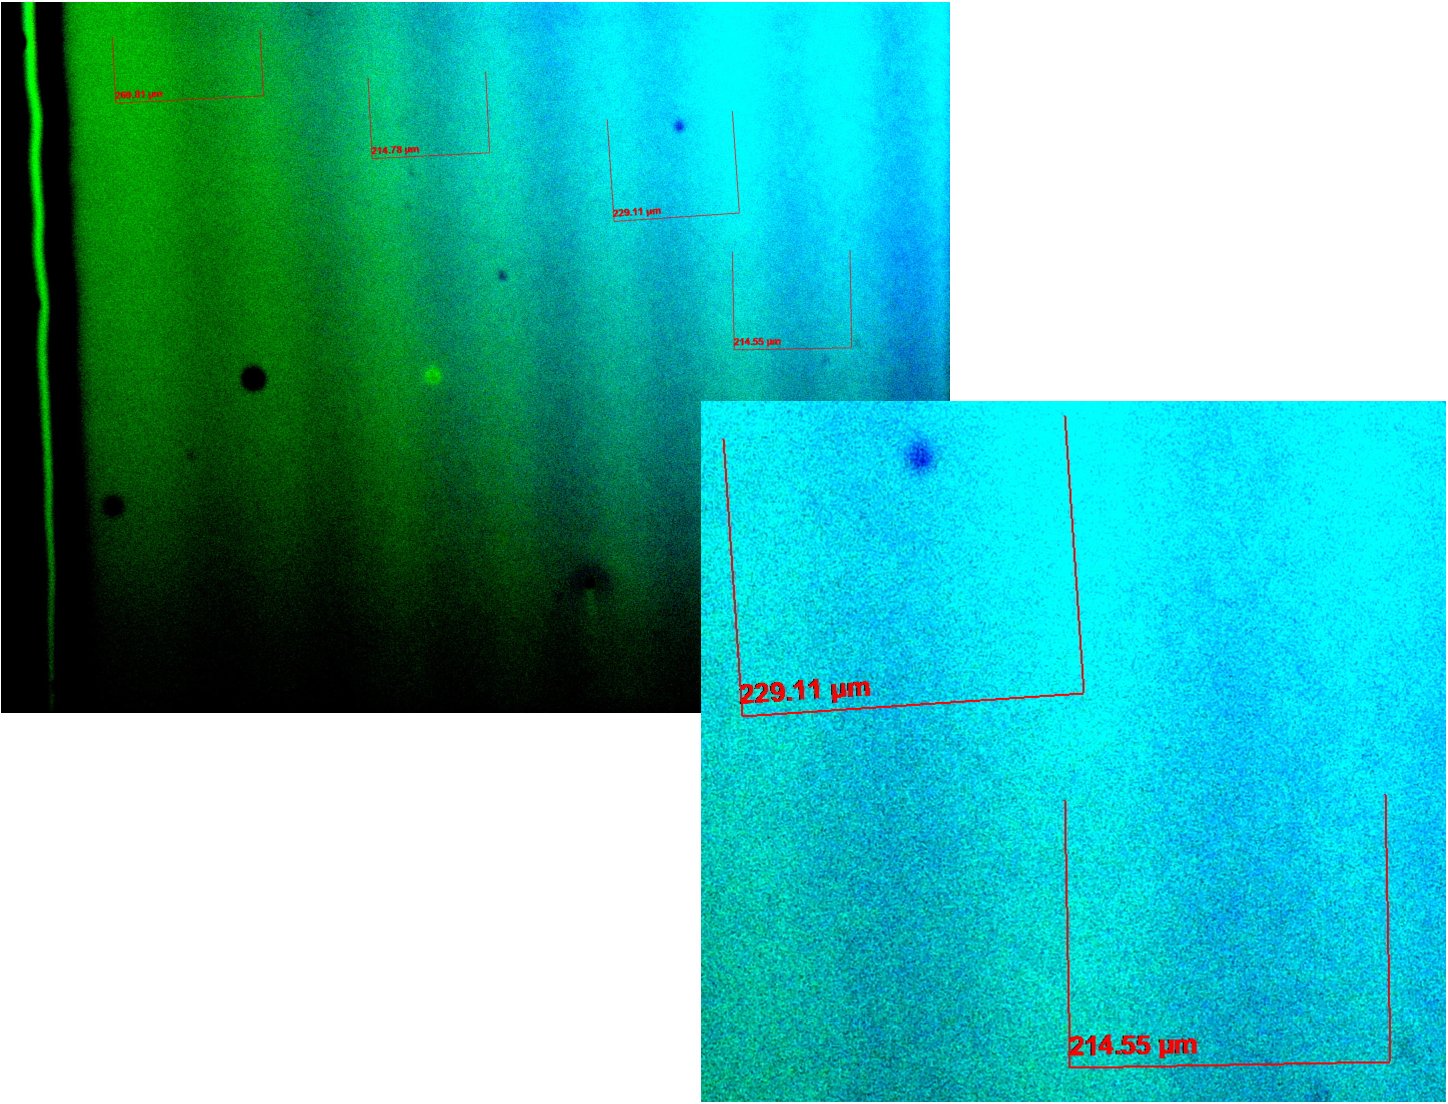
\psfig{file=chGratingProcess/zeiss_period.pdf,height=4.6in,width=6in}
\caption[High frequency structure in the photo resist]{High frequency structure in the photo resist color difference as probed by optical microscopy.  The Zeiss microscope at 5x shows a field of view a bit over 1.2 mm wide, showing subtle periodic waves in the resist thickness.  The period is in the range of 200-240 $\mu$m.  }
\label{fig:zeissfreq}
\end{center}
\end{figure}


\subsection{Uniformity along the slit}

\begin{tabular}{lccr}
\hline
Property & Symbol & Typical Value & Range \\
\hline
Motor angular rotation (rpm) & $\omega$ & 50 & 0$-$300 \\
Linear speed (mm/s) & $v$ & 4.2 & 0$-$25 \\
Translation screw pitch (tpi) & $\phi$ & 5 & $\cdots$ \\
%Motor resonant frequency (rpm) & $\omega_0$ & 60? & 43-67 \\
Vibration frequency (Hz) & $f_{vib}$ & 20 & 16-26 \\
RMS vibration amplitude (mm) & $<x>$ & 0.050 & 0.005-0.050 \\
Slit width (mm) & $w$ & 25 & 10$-$25 \\
Exposure time per pass (s) & $t$ & 6 & $>1$ \\
Dose to clear (passes) & $E_0$ & 14 & 14?$-$34? \\
Dose to clear (mJ/cm$^2$) & $E_0$ & 60? & 20?$-$100? \\

\hline
\end{tabular}

\begin{figure}[h!] 
\begin{center}
\ 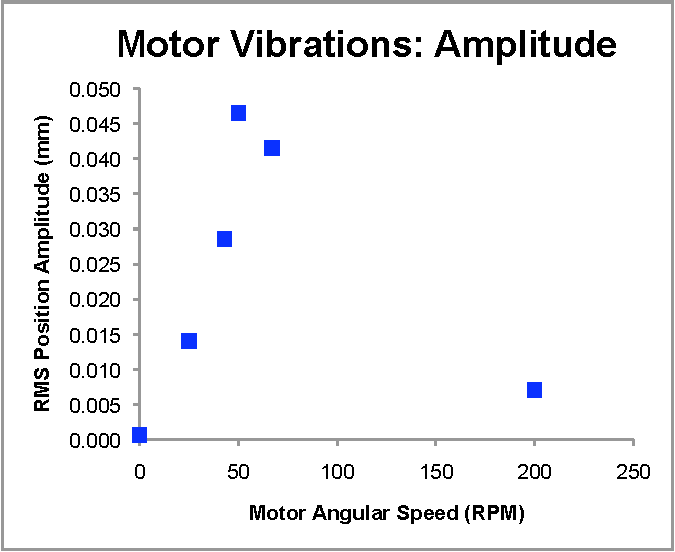
\psfig{file=chGratingProcess/resonantmotor.pdf,height=2.5in,width=3.5in}
\caption[Motor vibration amplitude]{RMS vibration amplitude as a function of driving frequency of the motor.}
\label{fig:resonantmotor}
\end{center}
\end{figure}

\begin{figure}[h!] 
\begin{center}
\ 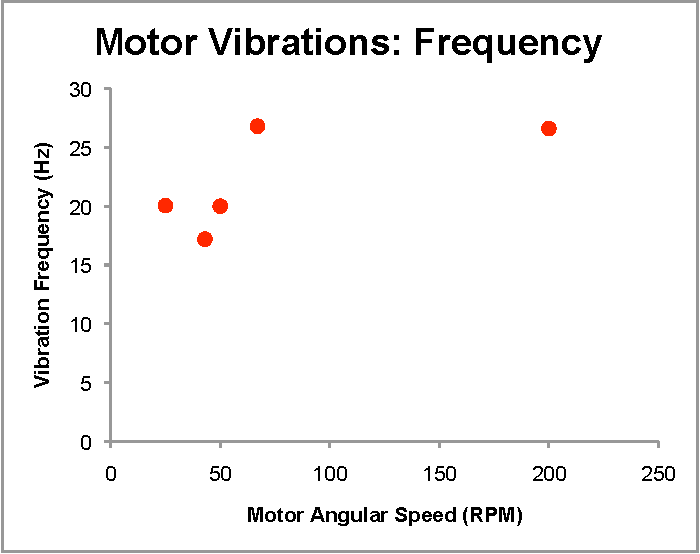
\psfig{file=chGratingProcess/freqresponse.pdf,height=2.5in,width=3.5in}
\caption[Motor vibration frequency]{Peak frequency of vibration as a function of driving frequency.  The power is almost entirely in the $x-$axis, which is the direction of motion of the car.}
\label{fig:freqresponse}
\end{center}
\end{figure}


\section{Anisotropic KOH etching}
Figure XX shows a schematic of the KOH etching process for the example of a biased wafer.
In principle, the KOH etching process should merely transfer the line edge positions from the Silicon Nitride hard mask into the silicon facets.  It is plausible that different etch rates over the surface will unevenly etch the surface, producing minute facet position differences.  One conceivable scenario is that the 30 mm thick Si puck has a different initial temperature from the surrounding bath.  The bath is typically either 40$\deg$ C or 68$\deg$ C.  The puck will warm from the edge to center, so that for the short duration of the temperature transition, the Si surface will experience increased etching at the edge.  Center-to-edge variations consistent with this type of over-etched edge pattern are conspicuous in interferometry of all our pieces (XX check the JPL piece).  The pattern is a focus aberration.  The amplitude of the focus aberration has a wide range among the dozen flat pieces with measured inter.  The clear strategy for mitigating the center-to-edge etch gradient is to equalize the part temperature and KOH solution temperature.

A similar center-to-edge etch gradient will occur if the etching rate is diffusion limited, and the circulation is better at the edge than at the center.  KOH etching in our process regime is generally temperature (XX) limited (cite XX -fundamentals of microelectronics), so the enhanced etch rate will be much smaller than the temperature gradient, but the diffusion gradient will last over the entirety of the etch process and not merely the beginning.

